\chapter{Cavo Coax}

\begin{figure}[h]
    \centering
    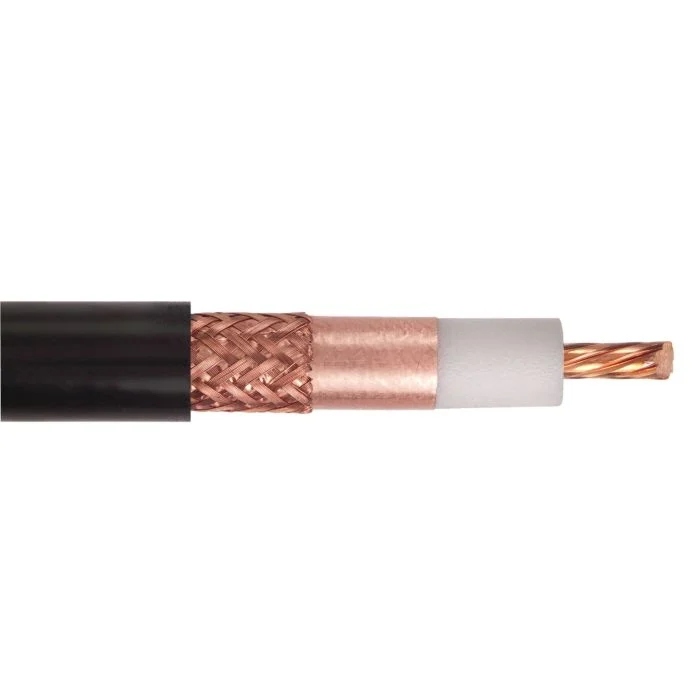
\includegraphics[scale = 0.5]{cavo coassiale vero.png}
\end{figure} 

\newpage 

\section{Campo EM in un cavo coax} 

\footnote{Slide del prof | PPT: Lezione 16 Mezzi trasmissivi 03 Maggio 23 | Pag 3-13}

\begin{figure}[h]
    \centering
    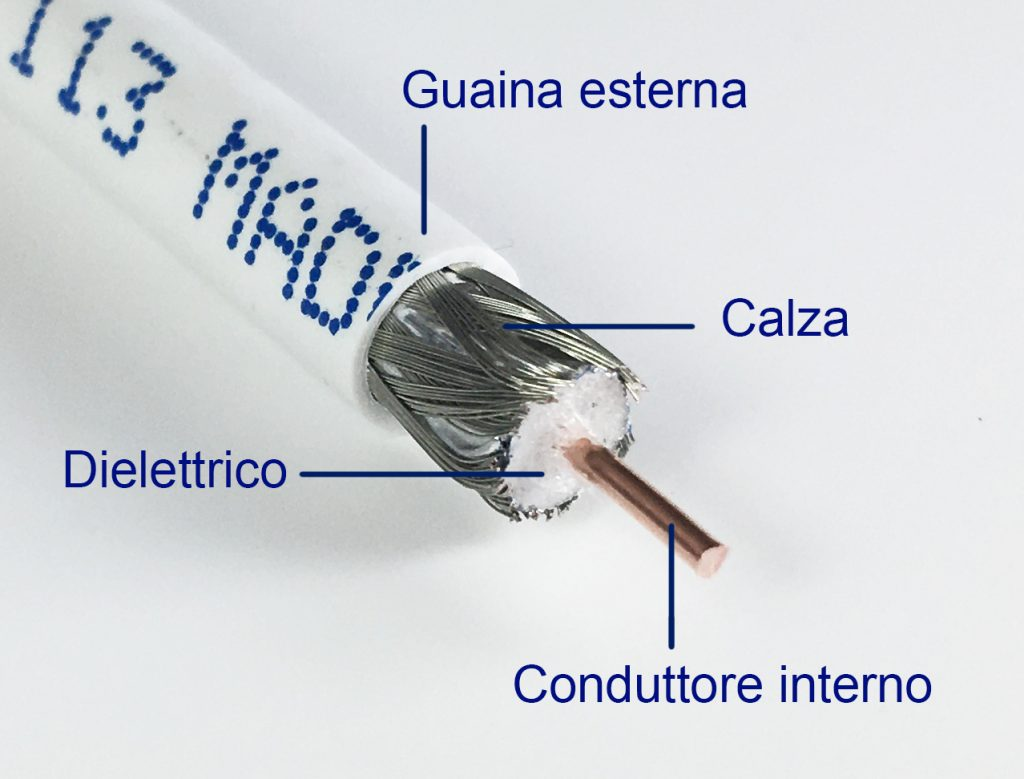
\includegraphics[scale = 0.5]{Cavo-spelato-nomi-delle-parti-copia-1024x779.jpg}
\end{figure} 

\footnote{\url{https://www.sistemi-integrati.net/cose-un-cavo-coassiale/}} 

Il cavo coassiale è un cavo cilindrico formato da (dall'interno all'esterno): 

\begin{itemize}
    \item condutore interno 
    \item dielettrico di separazione 
    \item calza conduttrice coassiale 
    \item guaina di protezione 
\end{itemize}

Essendo il cavo coassiale fisicamente di forma cilindrica, 
possiamo usare i fasori, in particolare le equazioni di Maxwell in forma 
fasoriale in assenza di sorgenti: 

{\Large \begin{equation}
    \begin{cases}
        \nabla \cdot \vec{E} = 0 \\ 
        \nabla \cdot \vec{H} = 0 \\
        \nabla \times \vec{E} = - \jmath \omega \mu \vec{H} \\ 
        \nabla \times \vec{H} = \jmath \omega \varepsilon \vec{E} 
    \end{cases}
\end{equation}}

Nella realtà non possiamo esprimere le equazioni delle onde in un cavo coassiale 
con le equazioni di Maxwell in assenza di sorgenti, ma adesso ci poniamo nel caso più 
semplice per svolgere i calcoli. \\ 

Sempre per quest'ultimo principio, consideriamo le onde polarizzate TEM, quindi: 

{\Large \begin{equation}
    \begin{cases}
        E_z = 0 \\ 
        H_z = 0
    \end{cases}
\end{equation}}

Considerando il cavo coassiale come cilindro, possiamo esprimere ogni punto del cavo 
in coordinate cilindriche: 

{\Large \begin{equation}
    (x, y, z) \Rightarrow (r, \phi, z )
\end{equation}}

\begin{tcolorbox}
    Dall'analisi matematica: 
    \begin{itemize}
        \item r indica il raggio 
        \item $\phi$ (si legge fi) indica i gradi  
    \end{itemize}
    Per approfondire\\
    \url{https://www.youmath.it/lezioni/analisi-due/varie/2282-coordinate-cilindriche.html} \\ 

    In questa sezione la notazione dei vettori indica quella di un fasore. 
\end{tcolorbox}

Vogliamo trovare una soluzione che non dipenda 
da $\phi$, quindi:
{\Large \begin{equation}
    \frac{\partial}{\partial \phi} = 0
\end{equation}} 

Essendo 
{
    \Large
     \begin{equation}
  E_z = 0      
     \end{equation}
}

$E_z$ è indipendete da $\phi$: 
questo principio prende il nome di simmetria azimutale. \\ 

Quindi possiamo scrivere che: 

{\Large \begin{equation}
    \nabla \cdot \vec{E} = 0 = \frac{1}{r} \frac{\partial}{\partial r} (r \vec{E_r} (r, z) )
\end{equation}}

Da questa equazione, notiamo che $\vec{E}$ dipende da r e da z. \\ 

Ritornando alla forma fisica del cavo coassiale, 
abbiamo due conduttori (il conduttore interno e la calza conduttrice coassiale) divisi 
da un dielettrico, proprio come un condensatore. \\ 

\begin{tcolorbox}
    Per approfondori sui condensatori \\
    \url{https://www.elettra2000.it/vdegliesposti/Dispense%20Propagazione/Richiami_Teoria_Dei_Circuiti.pdf}
\end{tcolorbox}
 
Applicando l'equazione costitutiva del condensatore al cavo coassiale, avremo che: 

{\Large \begin{equation}
    r \vec{E_r} (r, z) = Costante \cdot \vec{V} (z) 
    \Rightarrow \vec{E_r} (r, z) = \frac{Costante}{r} \vec{V} (z) 
\end{equation}}


\begin{figure}[h]
    \centering
    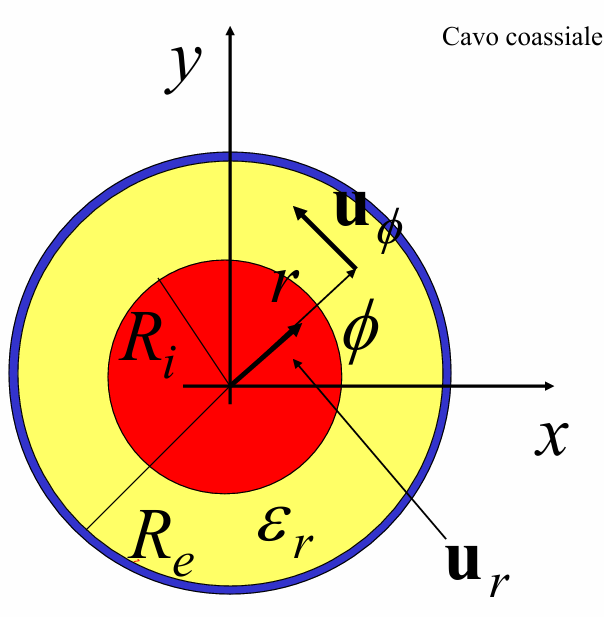
\includegraphics[scale = 0.5]{Cavo coax schematizzato.PNG}
\end{figure} 

\footnote{Slide del prof | PPT: Lezione 16 Mezzi trasmissivi 03 Maggio 23 | Pag 5} 

Proprio come il condensatore, facciamo un'intergrale di linea di un percorso chiuso tra le due armature, 
in questo caso tra i due conduttori: 

{\Large \begin{equation}
    \begin{split}
        \int_{R_i}^{R_e} \vec{E_r}(r, z) dr &= 
        \int_{R_i}^{R_e} \frac{Costante}{r} \vec{V} (z) dr \\
        & =  Costante \cdot \vec{V} (z) \int_{R_i}^{R_e} \frac{1}{r} dr \\ 
        & = Costante \cdot \vec{V} (z) \cdot \ln \left|r\right| \big|_{R_i} ^{R_e}   \\ 
        & =  Costante \cdot \vec{V} (z) \cdot \ln \left|R_e\right| - \\ 
        & Costante \cdot \vec{V} (z) \cdot \ln \left|R_i\right|  \\ 
        & = Costante \cdot \vec{V} (z) (\ln \left|R_e\right| - \ln \left|R_i\right|)  \\ 
        & = Costante \cdot \vec{V} (z) \ln \left|\frac{R_e}{R_i}\right|
    \end{split}
\end{equation}}

\begin{tcolorbox}
    $Costante \cdot \vec{V} (z)$ \\ 
    possiamo portarlo subito fuori dall'intergrale perchè 
    sono costanti rispetto a dr (r è l'incognita dell'integrale)   
\end{tcolorbox}

Alla fine avremo: 

{\Large \begin{equation}
    Costante \cdot \vec{V} (z) \ln \left|\frac{R_e}{R_i}\right| = \vec{V} (z)
\end{equation}}

Per essere vera questa ultima equazione: 

{\Large \begin{equation}
    Costante = \frac{1}{\ln \left|\frac{R_e}{R_i}\right|}
\end{equation}}

Sapendo ora il valore della costante possiamo esprimere $\vec{E_r}$ come: 

{\Large \begin{equation}
    \vec{E_r} (r, z) = \frac{Costante}{r} \vec{V} (z) 
    \Rightarrow \vec{E_r} (r, z) = \frac{1}{\ln \left|\frac{R_e}{R_i}\right|}  \frac{\vec{V} (z)}{r}
\end{equation}}

In "2.1 Equazioni dell'onda in forma fasoriale", abbiamo trovato che: 

{\Large \begin{equation}
    H_y = \frac{1}{- \jmath \omega \mu} \frac{\partial E_x}{\partial z}
\end{equation}}

In coordinate cilindriche, possiamo sostituire le rispettive coordinate, 
quindi $H_y$ diventa: 

{\Large \begin{equation}
    \vec{H_\phi} = \frac{1}{- \jmath \omega \mu} \frac{\partial E_r}{\partial z}
\end{equation}}

Sostitendo il valore di $\vec{E_r}$ trovato precedentemente, $\vec{H_\phi}$ diventa: 

{\Large \begin{equation}
    \vec{H_\phi} = \frac{1}{- \jmath \omega \mu} \frac{1}{r \ln \left|\frac{R_e}{R_i}\right| }\frac{\partial \vec{V} (z)}{\partial z}
\end{equation}}

Ritornando alle equazioni in forma fasoriale in coordinate cartesiane, sapevamo che: 

{\Large \begin{equation}
    \nabla \times \vec{H} = \jmath \omega \varepsilon \vec{E} 
    \Rightarrow \vec{E} = \frac{1}{\jmath \omega \varepsilon} \nabla \times \vec{H}
\end{equation}}

Sapendo il valore di $\vec{H}$, nell'asse x abbiamo che: 

{\Large \begin{equation}
    - \frac{\partial H_y}{\partial z} = \jmath \omega \varepsilon E_x 
    \Rightarrow E_x = - \frac{\partial H_y}{\partial z} \cdot \frac{1}{\jmath \omega \varepsilon}
\end{equation}}

Sostitendo a $x \Rightarrow r$ e $y \Rightarrow \phi$, avremo che: 

{\Large \begin{equation}
    \vec{E_r} (r, z) = - \frac{\partial H_\phi}{\partial z} \cdot \frac{1}{\jmath \omega \varepsilon}
\end{equation}}

Sapendo il valore di $H_\phi$, possiamo esprimere $\vec{E_r} (r, z)$ come: 

{\Large \begin{equation}
    \vec{E_r} (r, z) = - \frac{1}{r \ln \left|\frac{R_e}{R_i}\right|} \frac{1}{\kappa^{2}} \frac{\partial ^{2} \vec{V} (z)}{\partial  z^{2}}
\end{equation}}

Quindi è un'equazione che soddisfa l'equazione dell'onda: 

{\Large \begin{equation}
    \nabla ^{2} \vec{E} = -\kappa ^{2} \vec{E}
\end{equation}} 

dove: 

{\Large \begin{equation}
    \kappa ^{2} = \omega ^{2} \mu \varepsilon
\end{equation}} 

\newpage 

\section{Campo EM nel tempo}

\footnote{Slide del prof | PPT: Lezione 16 Mezzi trasmissivi 03 Maggio 23 | Pag 14 - 23}

Siccome le equazioni del campo EM soddisfano l'equazione dell'onda, 
possiamo esprimere la tensione come una sinusoide del tipo: 


{\Large  \begin{equation}
    \vec{E} (z) = V^{+} e^{-\jmath \kappa z} + V^{-} e^{+\jmath \kappa z}    
\end{equation}}


Ricordando che: 

{\Large \begin{equation}
    \vec{V} (z) = - \frac{1}{\kappa ^{2}} \frac{\partial^{2} \vec{V} (z)}{\partial z^{2}}
\end{equation}} 

e che: 

{\Large \begin{equation}
    \vec{E_r} (r, z) = \frac{1}{r \ln \left|\frac{R_e}{R_i}\right|} \vec{V}(z)
\end{equation}}

allora, possiamo convertire i fasori in quantità che variano nel tempo: 

{\Large \begin{equation}
    \begin{split}
        \Re{\vec{E_r} (r, z) e^{\jmath \kappa z}} 
        &= \frac{1}{r \ln \left|\frac{R_e}{R_i}\right|} \Re{\vec{V} (z) e^{\jmath \kappa z}} \\
        &= \frac{1}{r \ln \left|\frac{R_e}{R_i}\right|} V(z, t)
    \end{split}
\end{equation}}

dove: 

{\Large \begin{equation}
    \begin{split}
        V(z, t) 
        &=  \Re{\vec{V} (z) e^{\jmath \kappa z}} \\ 
        &= V^{+} \cos(\omega t - \kappa z) + V^{-} \cos(\omega t + \kappa z)     
    \end{split}
\end{equation}}

Come nel caso delle onde piane in forma fasoriale, possiamo descrivere V come somma 
di un'onda progressiva in direzione z e un'onda riflessa in direzione -z 

{\Large \begin{equation}
    \begin{split}
        V(z, t) &= f^{+} (t - \frac{z}{v}) + f^{-} (t + \frac{z}{v}) \\ 
        & = V^{+} \cos [\omega ( t - \frac{z}{v}) ] + V^{-} \cos [\omega ( t + \frac{z}{v}) ] 
    \end{split}
\end{equation}}

dove: 

{\Large \begin{equation}
    \begin{cases}
        v = \frac{\omega}{\kappa} 
        = \frac{\omega}{ \omega \sqrt{\mu \varepsilon}} 
        = \frac{1}{\sqrt{\mu \varepsilon}} 
        = c \\ 
        \lambda = \frac{2 \pi}{\kappa} 
        = \frac{2 \pi}{\omega} v 
        = \frac{v}{f}
    \end{cases}
\end{equation}}

Come le onde in forma fasoriale, $\vec{H_\phi}$ sarà: 

{\Large \begin{equation}
    \begin{split}
        \vec{H_\phi} &= \frac{1}{r \ln \left|\frac{R_e}{R_i}\right|} [V^{+} e^{-\jmath \kappa z} - V^{-} e^{\jmath \kappa z}] \\ 
        &= \sqrt{\frac{\varepsilon}{\mu}} \frac{1}{r \ln \left|\frac{R_e}{R_i}\right|} [V^{+} e^{-\jmath \kappa z} - V^{-} e^{\jmath \kappa z}]
    \end{split}
\end{equation}}

Come nelle onde piane, si può esprimere l'impedenza d'onda come: 

{\Large \begin{equation}
    \frac{\vec{E_r}^{+}}{\vec{H_\phi}^{+}} = 
    \sqrt{\frac{\mu_o}{\varepsilon}} = 
    \eta
\end{equation}}

Nel dominio del tempo $\vec{H_\phi}$ diventa: 

{\Large \begin{equation}
    \begin{split}
        \vec{H_\phi} (z, t) 
        &= \Re{\vec{H_\phi} e^{\jmath \omega t}} \\ 
        &= \sqrt{\frac{\varepsilon}{\mu}} \frac{1}{r \ln \left|\frac{R_e}{R_i}\right|} [V^{+} \cos(\omega t - \kappa z) - V^{-} \cos(\omega t + \kappa z)]
    \end{split}
\end{equation}} 

Sapendo ora il valore di $\vec{H_\phi}$,  
la corrente che fluisce nel conduttore interno è: 

{\Large \begin{equation}
    \begin{split}
        \vec{I} 
        &= \oint_{r = R_i} \vec{H_\phi} R_i d\phi \\
        &= \vec{H_\phi} \bigg|_{r = R_i} \cdot R_i \oint d\phi \\ 
        &= (\sqrt{\frac{\varepsilon}{\mu}} \frac{1}{r \ln \left|\frac{R_e}{R_i}\right|} [V^{+} \cos(\omega t - \kappa z) - V^{-} \cos(\omega t + \kappa z)]) \bigg|_{r = R_i} \cdot R_i \cdot 2\pi \\ 
        &= \sqrt{\frac{\varepsilon}{\mu}} \frac{1}{R_i \ln \left|\frac{R_e}{R_i}\right|} [V^{+} \cos(\omega t - \kappa z) - V^{-} \cos(\omega t + \kappa z)] \cdot R_i \cdot 2\pi \\ 
        &= 2\pi \sqrt{\frac{\varepsilon}{\mu}} \frac{1}{\ln \left|\frac{R_e}{R_i}\right|} [V^{+} \cos(\omega t - \kappa z) - V^{-} \cos(\omega t + \kappa z)] \\ 
        &=  I^{+} e^{- \jmath \kappa z} + I^{-} e^{+\jmath \kappa z}  
    \end{split}
\end{equation}} 

\begin{tcolorbox}
    Calcolare l'integrale di linea del percorso chiuso di un cerchio, in formula matematica \\ $\oint d\phi$ \\ 
    significa calcolare quanti radianti ci sono in un cerchio perchè l'incognita è 
    l'incognita $\phi$ e l'integrale è in $d\phi$. \\  \\ 
    Dalla geometria, i radianti di un qualsiasi cerchio, indipendentemente dal suo raggio, sono di $2 \pi$
\end{tcolorbox} 

\newpage 

\section{Costanti utili in un cavo coax} 

\footnote{Slide del prof | PPT: Lezione 16 Mezzi trasmissivi 03 Maggio 23 | Pag 24 - 29}

Una costante molto utile in un cavo coax  è la sua impedenza caratteristica: 

{\Large \begin{equation}
    \begin{split}
        Z_o 
        &= \frac{V^{+} e^{-\jmath \kappa z}}{I^{+} e^{-\jmath \kappa z}} = -\frac{V^{-} e^{+\jmath \kappa z}}{I^{-} e^{+\jmath \kappa z}} \\ 
        &= \frac{\sqrt{\frac{\mu}{\varepsilon}} \ln \left|\frac{R_e}{R_i}\right|}{2 \pi}
    \end{split}    
\end{equation}}

\begin{tcolorbox}
    Una piccola precisazione: \\ \\  
    l'impedenza caratteristica $Z_o$ dipende dalla tensione e dalla corrente 
    (da V e da I), quindi $Z_o$ dipende dal tipo di materiale utilizzato fisicamente nel cavo; \\ 
    a differenza dell'impendenza d'onda $\eta$ che dipende dal campo elettrico e dal campo magnetico 
    (da $\vec{E}$ e $\vec{H}$).      
\end{tcolorbox}


Quindi, possiamo esprimere la corrente in un punto z del cavo come: 
{\Large \begin{equation}
    \vec{I}(z)= \frac{1}{Z_o} [V^{+} e^{-\jmath \kappa z} - V^{-} e^{+\jmath \kappa z}]
\end{equation}} 

\begin{figure}[h]
    \centering
    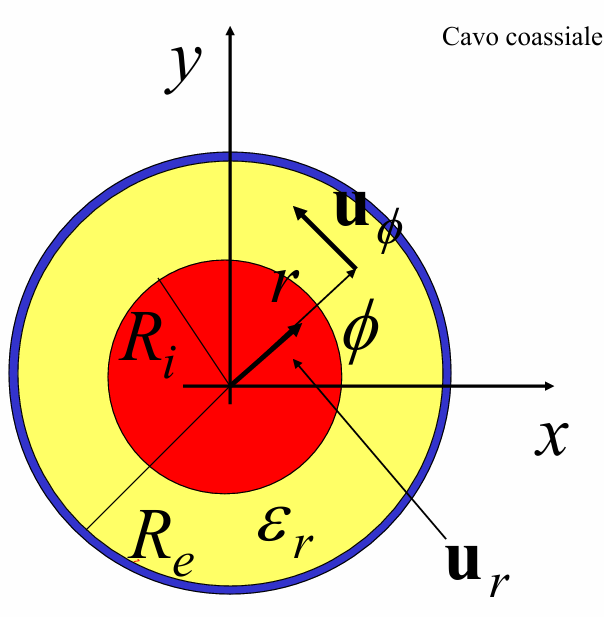
\includegraphics[scale = 0.5]{Cavo coax schematizzato.PNG}
\end{figure} 

\footnote{Slide del prof | PPT: Lezione 16 Mezzi trasmissivi 03 Maggio 23 | Pag 5} 

Visto che il cavo coassiale è formato da due conduttori, 
rispettivamente di raggio $R_i$ per il conduttore interno e di raggio $R_e$ per il conduttore esterno, 
divisi da un dielettrico, proprio come il condensatore, possiamo esprimere una carica per unità di lunghezza: 

{\Large \begin{equation}
    \begin{split}
        \hat{\rho_l} 
        &= \varepsilon \vec{E_r} (R_e, z) \hat{u_r} \cdot 2 \pi R_e \hat{u_r} \\ 
        &= \varepsilon \frac{1}{R_e \ln \left|\frac{R_e}{R_i}\right|} \vec{V} (z) \hat{u_r}  \cdot 2 \pi R_e \hat{u_r}
    \end{split}
\end{equation}}

dove l'unità di misura di $\hat{\rho_l}$ è: 

{\Large \begin{equation}
    [\hat{\rho_l} ] = \frac{C}{m}   
\end{equation}}

Proprio come il condensatore, possiamo esprimere la capacità per unità di lunghrzza come: 

{\Large \begin{equation}
    C = \frac{\hat{P_l}}{\hat{V} (z)} = \frac{2 \pi \varepsilon}{\ln \left|\frac{R_e}{R_i}\right|}
\end{equation}}

dove l'unità di misura di C è: 

{\Large \begin{equation}
    [C] = \frac{F}{m} 
\end{equation}} 

Essendo il cavo composto da due conduttori, possiamo esprimere il flusso di campo magnetico come: 

{\Large \begin{equation}
    \begin{split}
        \Phi_B 
        &= \mu_o \int_{R_i}^{R_e} \hat{H_\phi} dr \\  
        &= \mu_o \int_{R_i}^{R_e} \frac{\hat{I} (z)}{2 \pi} dr \\
        &= \mu_o \frac{\hat{I} (z)}{2 \pi} \ln \left|\frac{R_e}{R_i}\right| 
    \end{split}
\end{equation}} 

Quindi, possiamo esprimere l'induttanza per unità di lunghezza come: 

{\Large \begin{equation}
    L = \frac{\phi_B}{\hat{I}(z)} = \frac{\mu_o \ln \left|\frac{R_e}{R_i}\right|}{2 \pi}
\end{equation}}


Grazie ai valori di L e C, possiamo esprimere la velocità v, la costante di propagazione k e l'impedenza caratteristica $Z_o$: 

{\Large \begin{equation}
        Z_o = \sqrt{\frac{L}{C}} = \sqrt{\frac{\mu_o}{\varepsilon}} \frac{\ln \left|\frac{R_e}{R_i}\right| }{2 \pi} 
\end{equation}}

{\Large \begin{equation}
    v = \frac{1}{\sqrt{L C}} = \sqrt{\frac{2 \pi}{\mu_o \ln \left|\frac{R_e}{R_i}\right| } \cdot \frac{\ln \left|\frac{R_e}{R_i}\right|}{2 \pi \varepsilon}} = \frac{1}{\sqrt{\mu_o \varepsilon}}
\end{equation}} 

{\Large \begin{equation}
    \kappa = \omega \sqrt{L C} = \omega \sqrt{\mu_o \varepsilon}
\end{equation}}

\newpage 

\section{Teorema di Poynting in un cavo coax} 

\footnote{Slide del prof | PPT: Lezione 16 Mezzi trasmissivi 03 Maggio 23 | Pag 34-35}

Il teorema di Poynting è valido anche in un cavo coassiale. \\ 
Quindi, definiamo una superficie S ortogonale a $\hat{z}$: 

{\Large \begin{equation}
    \begin{split}
        \vec{S} 
        &= \vec{E} \times \vec{H}^{*} \\ 
        &= \frac{\hat{r} V(z)}{r \ln \left|\frac{R_e}{R_i}\right|}  \times \frac{\hat{\phi}}{2 \pi r} I^{*} (z) \\ 
        &= \frac{\hat{z}}{2 \pi r^{2} \cdot \ln \left|\frac{R_e}{R_i}\right|} V(z) I^{*} (z) 
    \end{split}
\end{equation}}

Dato S, possiamo calcolarci la potenza attiva trasportata da un'onda TEM in un cavo coax: 

{\Large \begin{equation}
    \begin{split}
        P &= \frac{1}{2} \Re{\int \int \vec{S} \cdot \hat{z} ds} \\ 
        &= \frac{1}{2} \Re{\int_{0}^{2 \pi} \int_{R_i}^{R_e} \vec{S} \cdot \hat{z} r dr d\phi} \\
        &= \frac{1}{2} \Re{V(z) I^{*} (z)} \\ 
        &= \frac{1}{2 Z_o} (\left|V^{+}\right| ^{2} - \left|V^{-}\right| ^{2})
    \end{split}
\end{equation}}

\newpage 

\section{Perdite nel dielettrico} 

\footnote{Slide del prof | PPT: Lezione 20 Perdite nel dieletrico 17 maggio 23 | Pag 3-4}

I due conduttori che costituiscono un cavo coax sono tenuti da un dielettrico con bassa permeattività 
(ad esempio il telflon). \\ 

\begin{tcolorbox}
Da \url{https://it.wikipedia.org/wiki/Permittivit%C3%A0_elettrica} \\
La permittività elettrica è una grandezza fisica che quantifica la tendenza del materiale a contrastare l'intensità del campo elettrico presente al suo interno. Descrive quindi il comportamento di un materiale in presenza di un campo elettrico. Viene anche comunemente chiamata costante dielettrica. \\ \\ 
La permittività elettrica è fortemente legata alla suscettività elettrica, ovvero alla predisposizione del materiale a polarizzarsi quando viene applicato un campo elettrico. La polarizzazione di atomi e molecole produce un campo elettrico aggiuntivo nel materiale, descritto attraverso il vettore induzione elettrica, e la permittività elettrica ne quantifica l'entità per unità di carica elettrica.    
\end{tcolorbox}

Quindi, il campo elettrico tra questi due conduttori è: 

{\Large \begin{equation}
    \vec{D} = \varepsilon_o \vec{E} + \vec{P_l}
\end{equation}}
 
dove $\vec{P_l}$ è la perdita del campo elettrico nel dielettrico. \\ \\ 

Se il mezzo è lineare: 

{\Large \begin{equation}
    \vec{P_l} = \varepsilon_o \chi_e \vec{E}
\end{equation}} 

\begin{tcolorbox}
    $\chi$ lettera greca che si legge chi
\end{tcolorbox}

dove $\chi_e$ tiene conto dell'energia EM dissipata sotto forma di calore. \\ \\ 

Permeattività complessa: 

{\Large \begin{equation}
    \begin{split}
        \varepsilon 
        &= \varepsilon_o (1 + \chi_e) \\ 
        &= \varepsilon_o \varepsilon_r (1 - \jmath \tan \delta)
    \end{split}
\end{equation}}

\begin{tcolorbox}
    $\delta$ lettera greca che si legge delta
\end{tcolorbox}

dove: 

$\delta$ è un parametro del dielettrico e non dipende dalla profondità di penetrazione. 

\begin{tcolorbox}
    Da \url{https://www.scienzaatscuola.it/fisica%205g/vivente3.html} \\ 
    La quantità $\delta$ è detta profondità di penetrazione e indica la distanza alla quale i campi si sono ridotti a circa il 37\% e la densità di potenza si è ridotta a meno del 14\% rispetto ai valori all'interfaccia. 
\end{tcolorbox}

Sapendo $\delta$, possiamo esprimere $\kappa$ come: 

{\Large \begin{equation}
    \begin{split}
        \kappa 
        &= \omega \sqrt{\mu_o \varepsilon} \\ 
        &\approx \omega \sqrt{\mu_o \varepsilon_o \varepsilon_r } (1 - \jmath \frac{\tan \delta}{2})    
    \end{split}
\end{equation}}

Inoltre, possiamo esprimere una costante di attenuazione del dielettrico $\alpha_d$ come: 

{\Large \begin{equation}
    \alpha_d \approx \kappa \frac{\tan \delta}{2}
\end{equation}}

Oltre al dielettrico, il cavo coax presente due conduttori, quindi possiamo 
esprimere una costante di attenuazione del conduttore $\alpha_c$ come: 

{\Large \begin{equation}
    \begin{split}
        \alpha_c 
        &= \frac{P_l (z)}{2P(z)} \\ 
        &\approx \frac{\frac{R_s}{4 \pi} [\frac{1}{R_i} + \frac{1}{R_e}]}{Z_o} \\ 
        &= \frac{\frac{R_s}{4 \pi R_i} [1 + \frac{R_i}{R_e}]}{\frac{\eta}{2 \pi} \ln \left|\frac{R_e}{R_i}\right|}
    \end{split}
\end{equation}} 

dove: 

{\Large \begin{equation}
    \begin{cases}
        R_s = \frac{1}{\sigma \delta} \\ 
        \sigma = \frac{1}{\sqrt{\pi f \mu_o \sigma}}
    \end{cases}
\end{equation}}

\begin{tcolorbox}
    $\sigma$ lettera greca si legge sigma
\end{tcolorbox}

Spesso, è preferibile esprimere le perdite totali in un cavo coax in dB: 

{\Large \begin{equation}
    \alpha_{dB} = -20 \log e^{- (\alpha_c + \alpha_d)}
\end{equation}} 

\newpage 

\section{Perdite dipendenti dalla temperatura nel dielettrico}

\footnote{Slide del prof | PPT: Lezione 20 Perdite nel dieletrico 17 maggio 23 | Pag 15}

La temperatura influisce sul coefficiente elettrico di attenuazione $\alpha(T)$: 

{\Large \begin{equation}
    \alpha (T) = \alpha_{293 K} \cdot \sqrt{1 + \sigma_P (\frac{T}{K} - 293)}
\end{equation}}


dove: 
\begin{itemize}
    \item $\alpha_P$ è il coefficiente di resistività (è un parametro empirico riguardo al materiale del conduttore) 
    \item $\alpha_{293 K}$  è la resistività a 293 Kelvin 
\end{itemize}

Se il cavo coax è corto circuitato: 

{\Large \begin{equation}
    V^{+} = -V^{-}
\end{equation}} 

Quindi: 

{\Large \begin{equation}
    V_{max} = 2 \left|V^{+}\right|
\end{equation}}

\newpage 
